% <BNAIC-STYLE>
\documentclass{article}
\usepackage{bnaic}
\usepackage{todonotes}
\usepackage{svg}
\usepackage{float}
\usepackage{caption}
\usepackage{subcaption}

\usepackage{hyperref}
\usepackage{amsmath}
\usepackage{amsfonts}

\usepackage{array}
\usepackage{wrapfig}

%% if your are not using LaTeX2e use instead
%% \documentstyle[bnaic]{article}

%% begin document with title, author and affiliations

\title{\textbf{\huge Making Art with Generative Adversarial Networks}}
\author{Loran Knol (s3182541)\affila \and Thijs Havinga (s2922924)\affila \and Elisa Oostwal (s2468255) \affila \and Jeroen Overschie (s2995697) \affila \and}
\date{\affila\ \textit{University of Groningen, Nijenborgh 9 9747AG Groningen}}

\pagestyle{empty}

\begin{document}
\ttl
\thispagestyle{empty}

\begin{abstract}
\noindent
Generative Adversarial Networks (GANs) have proven fit to generate increasingly realistic images, or, for instance, copy the style of one piece of art (typically a painting) to another. A number of recent developments have shown very promising results, such as the progressively growing StyleGAN \cite{karras2019stylebased} that generates images of human faces with high resolution. This study aims to use those developments to generate paintings with the style and content of just one painter, namely the Dutch Vincent van Gogh. Although this painter was productive, the number of usable paintings was still too small for training GANs, so data augmentation had to be performed. Two different architectures, namely DCGAN and StyleGAN were trained on the augmented data. Of the two, StyleGAN showed the most promising results.
\end{abstract}
% </BNAIC-STYLE>

% <NON-BNAIC STYLE>
% \documentclass{article}
% \usepackage[english]{babel}
% \usepackage{palatino,mathpazo}
% \usepackage[utf8]{inputenc}
% \setlength\parindent{0pt}
% \pagenumbering{gobble}
% \usepackage[margin=1.4in]{geometry}

% \usepackage[maxnames=20]{biblatex}
% \usepackage{csquotes}
% \addbibresource{bibliography.bib}
% \usepackage[nottoc,numbib]{tocbibind}

% \usepackage{graphicx}
% \usepackage{amssymb}
% \usepackage{amsmath}

% % Lame title idea: Faking Van Gogh :')
% % pretty nice title 

% \title{Making Art with Generative Adversarial Networks}
% \author{Loran Knol (s3182541)\\Thijs Havinga (s2922924)\\Elisa Oostwal (s2468255)\\Jeroen Overschie (s2995697)}
% \date{\today}

% \begin{document}

% \maketitle
% </NON-BNAIC STYLE>

\section{Introduction}
% <COPIED FROM PROPOSAL> 

% Elisa: maybe largely delete the first paragraph to save space?

% About Generative Adversarial Networks
Generative Adversarial Networks are a relatively new type of technique, in which two networks are simultaneously trained whilst competing against each other. One of the networks is a \textit{generative} network, which generates new 'candidates' from a lower-dimensional space, trying to represent the data distribution of interest. A candidate could, for example, be a picture of a person or some other entity. The other network, however, is of a \textit{discriminative} type, which tries to classify the candidates produced by the generative network as either real or fake. As such, the two networks play a zero-sum game: the generative network tries to ``fool'' the discriminative network, while the discriminative network tries to tell real from synthesized. The generative network is thus stimulated to create ever more convincing candidates, up to a level where it might be impossible to tell real from fake.\\

% Short description of the project / project goal + Datasets / simulator used
In this project, we aim to train such a Generative Adversarial Network ourselves, with the purpose of image generation specifically. As the generation of human faces has been widely studied, we have chosen a different topic, namely, the generation of paintings. While large datasets of paintings are available (e.g., ~\cite{kaggle_rijksmuseum}), we have opted to restrict ourselves to one artist, as we believe this will give a better chance at producing realistic paintings. For this, we have chosen the Dutch artist Vincent van Gogh, who is known for his unique style. The dataset is taken from~\cite{kaggle_van_gogh} and consists of roughly $2 \times 10^3$ images. The goal then becomes to generate paintings that resemble Van Gogh's in terms of color usage and style.\\
% </COPIED FROM PROPOSAL>

\section{Generative Adversarial Networks}\label{sec:GANs}
Generative models have been existent in Machine Learning literature for some time - we are able to draw samples from distributions using sampling techniques such as rejection sampling or Markov Chain Monte Carlo techniques such as Gibbs sampling. However, we are often obliged to make harsh assumptions about the data distribution at hand: obstructing the goal of wanting to learn and generate more samples from a distribution automatically. Whereas discriminative models have seen massive successes in the Deep Learning world \cite{hinton2012deep}, generative models enjoyed success a bit later.

Generative models preceding GAN's include denoising Auto-encoders \cite{lu2013speech}, Deep Boltzmann Machines \cite{salakhutdinov2009deep} or Generative Stochastic Networks \cite{bengio2014deep}. Whereas Deep Boltzmann Machines use an undirected graphical model approach with latent variables, Generative Stochastic Networks do not require a Machine Learning practitioner to define an explicit distribution - allowing training by using ordinary back-propagation. Auto-encoders also use a latent code using a deep network - forcing the model to compress the essential data distribution information into the bottleneck latent code layer. After the input data was 'compressed' into a smaller latent code layer, the auto-encoder will decode the latent code, trying to best reconstruct the original input.

\textit{Generative Adversarial Models} \cite{goodfellow2014generative} add another component: the \textbf{adversary}. Whilst the Generating model $G$ tries to best reconstruct a sample matching the original data distribution from just a latent code, the Adversarial discriminative model $D$ will try to classify the generated output as real of fake in a zero-sum game. In this way, we train two models simultaneously with opposing goals: whilst $G$ wants to best 'fool' the discriminator, $D$ wants to best classify whether a sample is made by $G$ and is in $p_G$ or whether it came from the real data distribution $x$. Given some noise input $z$ drawn from $p_z$, $G$ wants to minimize $\log(1-D(G(z)))$. The game $D$ and $G$ play can be formalized as:

\begin{equation}\label{gan-objective-function}
\min _{G} \max _{D} V(D, G) = \mathbb{E}_{\boldsymbol{x} \sim p_{\text {data }}(\boldsymbol{x})}[\log D(\boldsymbol{x})]+\mathbb{E}_{\boldsymbol{z} \sim p_{\boldsymbol{z}}(\boldsymbol{z})}[\log (1-D(G(\boldsymbol{z})))]
\end{equation}

Which means our objective/loss function is a combination of two models: one trying to minimize some quantity whilst the other is trying to maximize it. Note that Equation~\ref{gan-objective-function} might be modified to prevent gradient saturation - we might instead train $G$ to maximize $\log D(G(z))$. Though GAN's can be effectively trained using this formulation, we are at the risk that one model might excel over the other. In this case training effectiveness will falter - causing the zero-sum game dynamics to fail. Contemporary GAN's often take extra measures to best synchronize $D$ and $G$ during training.

\section{Data}

The dataset used in our study is taken from~\cite{kaggle_van_gogh}. This collection consists of approximately $2 \times 10^3$ paintings by Van Gogh. Upon further inspection we find that the set contains both black-and-white sketches as well as colored paintings. To aid the specialization of the network we opt to only use the colored paintings for training, filtering the images based on high saturation. This reduces the number of images to ... . This is a rather small number of samples, considering usually ten-thousands or even millions of images are used in order to train a GAN, see e.g.~\cite{radford2015unsupervised}. We therefore resolve to data augmentation in order to increase the number of images. The details of this are described in the following subsection.

\subsection{Data augmentation}

From our data set, we  generate square patches as data samples for our GAN model. Through various methods, we produce square pictures of a fixed size in pixels. This makes it easier to use the samples in a model. Using various methods, we generate patches that are sligthly different while retaining the visual contents of the painting. The methods used, in order, are:
\begin{enumerate}
    \item Adjusting the brightness of the picture by -5\%, 0\% or 5\%.
    \item Applying a \emph{shear} operation on the picture in the x- and/or y-axis, or neither.
    \item From the resulting pictures, cutting square patches that cover as much of the picture as possible. This yields several possible square sub-images.
    \item Resizing the square patches to a fixed size (for example, $212 \times 212$).
    \item To the resulting patch, some noise from a normal distribution ($\sigma = 5$ for integer pixel values) can be added or not.
\end{enumerate}
All of these steps together produce a large number of possible slightly different visual patches from the same painting. Figure~\ref{fig:data_aug} shows some examples of patches that are generated from a single painting.

% Elisa: maybe remove this figure to save space?

\begin{wrapfigure}{r}{0.4\linewidth}
    %\centering
    \begin{subfigure}[b]{0.3\linewidth}
        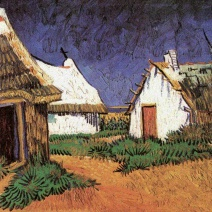
\includegraphics[width=\textwidth]{report/img/data_aug/19597.jpg}
    \end{subfigure}
    \hfill
    \begin{subfigure}[b]{0.3\linewidth}
        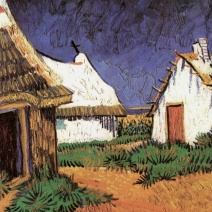
\includegraphics[width=\textwidth]{report/img/data_aug/19612.jpg}
    \end{subfigure}
    \hfill
    \begin{subfigure}[b]{0.3\linewidth}
        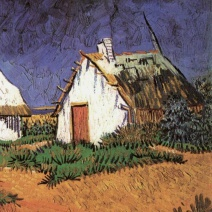
\includegraphics[width=\textwidth]{report/img/data_aug/19616.jpg}
    \end{subfigure}
    \hfill
    % \begin{subfigure}[b]{0.15\textwidth}
    %     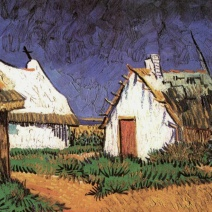
\includegraphics[width=\textwidth]{report/img/data_aug/19626.jpg}
    % \end{subfigure}
    % \hfill
    % \begin{subfigure}[b]{0.15\textwidth}
    %     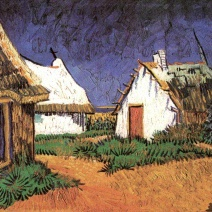
\includegraphics[width=\textwidth]{report/img/data_aug/19637.jpg}
    % \end{subfigure}
    % \hfill
    % \begin{subfigure}[b]{0.15\textwidth}
    %     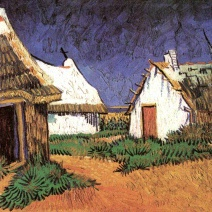
\includegraphics[width=\textwidth]{report/img/data_aug/19645.jpg}
    % \end{subfigure}
    % \begin{subfigure}[b]{0.15\textwidth}
    %     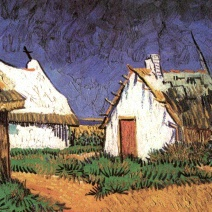
\includegraphics[width=\textwidth]{report/img/data_aug/19659.jpg}
    % \end{subfigure}
    % \hfill
    % \begin{subfigure}[b]{0.15\textwidth}
    %     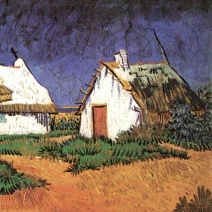
\includegraphics[width=\textwidth]{report/img/data_aug/19667.jpg}
    % \end{subfigure}
    % \hfill
    % \begin{subfigure}[b]{0.15\textwidth}
    %     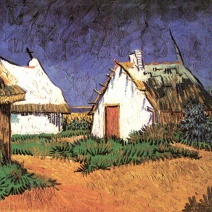
\includegraphics[width=\textwidth]{report/img/data_aug/19675.jpg}
    % \end{subfigure}
    % \hfill
    % \begin{subfigure}[b]{0.15\textwidth}
    %     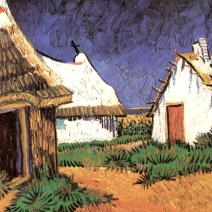
\includegraphics[width=\textwidth]{report/img/data_aug/19684.jpg}
    % \end{subfigure}
    % \hfill
    % \begin{subfigure}[b]{0.15\textwidth}
    %     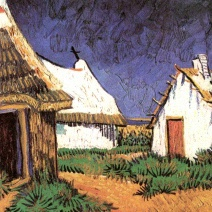
\includegraphics[width=\textwidth]{report/img/data_aug/19693.jpg}
    % \end{subfigure}
    % \hfill
    % \begin{subfigure}[b]{0.15\textwidth}
    %     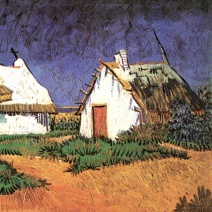
\includegraphics[width=\textwidth]{report/img/data_aug/19703.jpg}
    % \end{subfigure}
    \caption{Examples of visual patches as produced by our data augmentation routine from a single source painting.}
    \label{fig:data_aug}
\end{wrapfigure}

\section{Methods}

\subsection{DCGAN}
Described in \cite{radford2015unsupervised}, the DCGAN model refers simply to using deep convolutational networks for a GAN architecture. As a first experiment to use our augmented data set, we create a design from scratch from the two essential components in a GAN, the generator network $G$ and the discriminator network $D$. We also added an encoder component $E$ later to better allow the generator to learn useful weights: Training this additional encoder network with the generator network as an autoencoder based on the same data set allows these networks to learn latent representations which the generator is able to translate to the original paintings. By using a subset of 3 paintings from the original data set and applying our data augmentation routine, we attain our final data set $X$ for use in our DCGAN. Training the combination of $E$ and $G$ with $X$ as both the input and the expected output, $E$ learns to generate latent representations $h$ from samples from $X$, while $G$ learns to transform $h$ back to the original sample. At the same time, $G$ and $D$ are trained with zero-sum adversarial optimizer functions as described in Section~\ref{sec:GANs}. As such, $D$ learns to distinguish output from $G$ produced with any random latent code from original data samples from $X$, while $G$ learns to generate pictures that look increasingly like the data samples.

\begin{wrapfigure}{r}{0.8\linewidth}
    \centering
    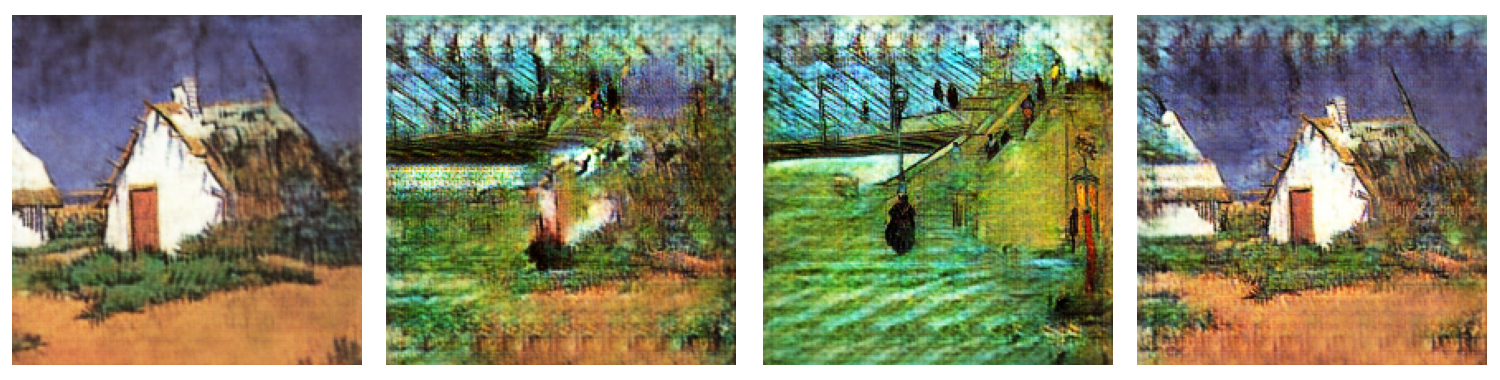
\includegraphics[width=\linewidth]{report/img/dcgan2.png}
    \caption{Example results from our DCGAN architecture. The left-most picture was generated with a latent code produced by the encoder and thus represents one of the input samples. The remaining pictures were generated from random latent codes.}
    \label{fig:dcgan}
\end{wrapfigure}

\subsection{StyleGAN}
Aside from DCGAN, a more recently developed GAN architecture called StyleGAN \cite{karras2019stylebased} was also used. StyleGAN is based on Progressive GAN \cite{karras2018progressive}, which, for both the generator and discriminator components, adds layers during training, yielding generated images of increasingly higher resolution. This progressive growing of image resolution is beneficial for both speeding up and stabilizing the training process. StyleGAN, in turn, modifies the architecture grown by Progressive GAN in a number of ways. 

The first modification concerns the latent code, $\mathbf{z} \in \mathcal{Z}$, which is not fed directly to the network but is first pre-processed by an eight-layered fully connected (FC) multi-layer perceptron (MLP) $f$ to produce the intermediate latent vector $\mathbf{w} \in \mathcal{W}$. Learned affine transformations $A$ then convert $\mathbf{w}$ to so-called styles $\mathbf{y} = (\mathbf{y}_s, \mathbf{y}_b)$, which in turn are fed into adaptive instance-normalization (AdaIN) units. With this set-up, the AdaIN units instance-normalize the feature maps $\mathbf{x}_i$ of a second input $\mathbf{x}$, rescale the normalized input with $\mathbf{y}_s$ and finally shift the instance-normalized, rescaled $\mathbf{x}$ with $\mathbf{y}_b$: 

\begin{equation}
    \text{AdaIN}(\mathbf{x}_i, \mathbf{y}) = \mathbf{y}_{s,\, i} \frac{\mathbf{x}_i - \mu(\mathbf{x}_i)}{\sigma(\mathbf{x_i})} + \mathbf{y}_{b,\, i},
\end{equation}

\noindent
ensuring the mean and variance of every feature map $\mathbf{x}_i$ become aligned with the style $\mathbf{y}_i$ \cite{huang2017arbitrary, karras2019stylebased}.

As a final modification, StyleGAN injects independent images of Gaussian noise after every convolutional layer, before the input is fed into the AdaIN units. The noise is scaled per channel with a learned transformation $B$, and is hypothesized to relieve the network from the burden of having to generate its own pseudorandom numbers from the network input to induce the necessary stochasticity at the different resolution levels in the generated images \cite{karras2019stylebased}. See Figure \ref{fig:stylegan_architecture} for an overview of the StyleGAN architecture.

% Resize this figure at some point
\begin{wrapfigure}{r}{0.4\linewidth}
    \centering
    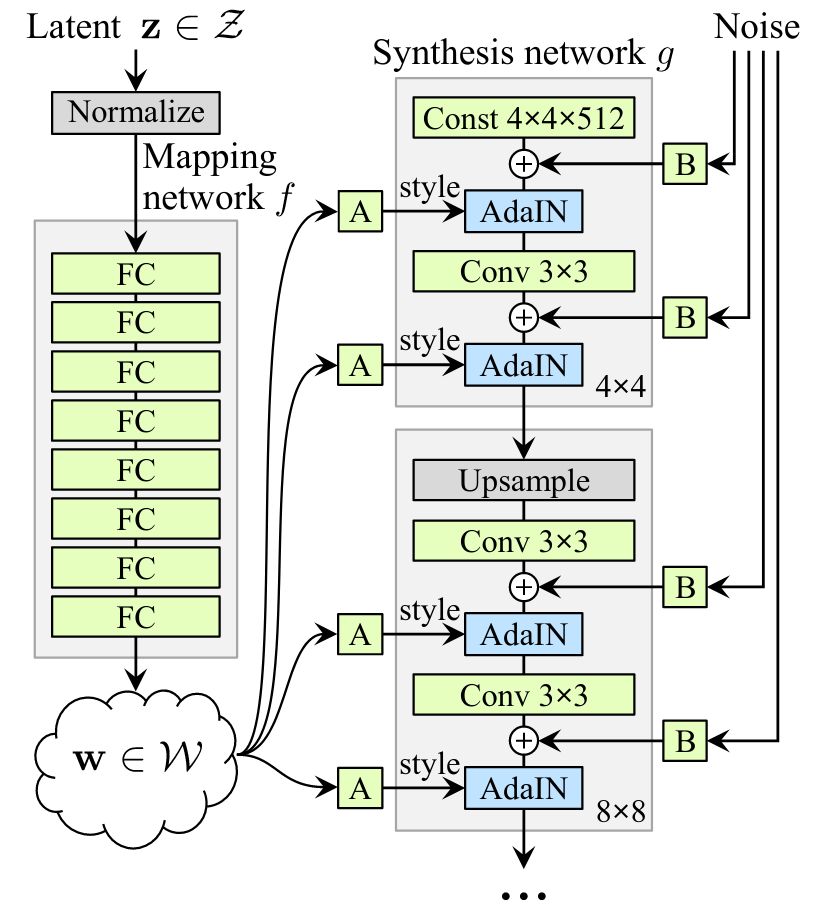
\includegraphics[width=\linewidth]{report/img/stylegan_architecture.png}
    \caption{StyleGAN architecture. A latent code $\mathbf{z}$ is transformed through the MLP $f$ to $\mathbf{w}$, which then controls the AdaIN units within the generator $g$. Independent noise images are injected before every AdaIN unit. Every block of two convolutional layers (and their respective AdaIN units) is responsible for upsampling the image from the previous block; the resulting resolution is indicated in the lower-right corner of the gray outlines. Taken from \cite{karras2019stylebased}.}
    \label{fig:stylegan_architecture}
\end{wrapfigure}

Because the training of StyleGAN takes a considerable amount of time and it was unsure whether the training method would converge within the given time constraints, two separate approaches were taken. The first one takes a StyleGAN instance from \cite{karras2019stylebased} that was fully trained on a high-quality (resolution: 1024x1024) faces dataset. With that fully trained network, training is then continued on the augmented Van Gogh dataset. This means that the network does not grow in resolution anymore, since the maximum resolution (1024x1024) has already been reached before the Van Gogh training even commenced. The intuition behind this approach is that the faces generated by the original StyleGAN instance hopefully already lie closer to the manifold of Van Gogh paintings than the pure noise images an untrained instance would generate, especially given the fact that Van Gogh has drawn quite a lot of (self-)portraits.

The second approach is somewhat similar to the first one, in that a fully trained, face generating StyleGAN instance is used as a basis. However, contrary to the first approach, all training parameters are reset to their starting values - including the resolution. The high-resolution layers are not removed, but they are simply disregarded as long as the resolution has not grown to the required size. This allows the parameters of the low-resolution parts of the original, fully trained network to be retrained first. Only then will the parameters of higher-resolution parts be retrained. In other words, whereas the first approach makes use of transfer learning with a constant network size, the second approach combines both transfer learning and progressive growing.

The training hyperparameters were kept the same as in \cite{karras2019stylebased}. The network was trained with non-saturating GAN loss, using the Adam optimizer \cite{kingma2017adam} with $\alpha = 0.001$, $\beta_1 = 0$, and $\beta_2 = 0.99$. However, $\alpha$ increased with resolution size, and its values were 0.0015 for $128^2$, 0.002 for $256^2$, 0.003 for $512^2$ and $1024^2$. The minibatch size also varied per resolution: 256 for $4^2$ and $8^2$, 128 for $16^2$, 64 for $32^2$, 32 for $64^2$, 16 for $128^2$ and 8 for $256^2$, $512^2$, and $1024^2$.

Both networks were trained with two NVIDIA Tesla K40 GPUs and a total of 24 cores from two Intel Xeon E5 2680v3 CPUs; each network received 24 hours of training. The results of both networks will be compared qualitatively, primarily based on how much the authors think the generated images resemble Van Gogh paintings, and quantitatively, which incorporates calculating the Fréchet Inception Distance (FID) \cite{heusel2017frechet} with an Inception-v3 network \cite{szegedy2016inception} that has been trained on ImageNet \cite{imagenet2009}.

\section{Results}

\subsection{StyleGAN}
A sample of the images generated by the StyleGAN instance with constant network size (also referred to as `training resumed' from here) over the course of training is given in Figure \ref{fig:sample_resumed}. Every row corresponds to a random latent code, every column to the network state at the end of a training tick. The number of images the network needs to be trained on before one tick has passed depends on the training schedule; such a tick thus does not necessarily constitute one full pass through the training data (i.e. a tick is not an epoch). The first column in the figure contains images generated by the original StyleGAN instance from \cite{karras2019stylebased}. From the second column onward, the originally generated faces quickly get a painting-like look and morph into objects that Van Gogh would often paint, like flowers and (self-)portraits. However, the very last column contains images that do not seem to match the painting style and objects observed in the middle four columns.

\begin{wrapfigure}{R}{0.5\linewidth}
    \centering
    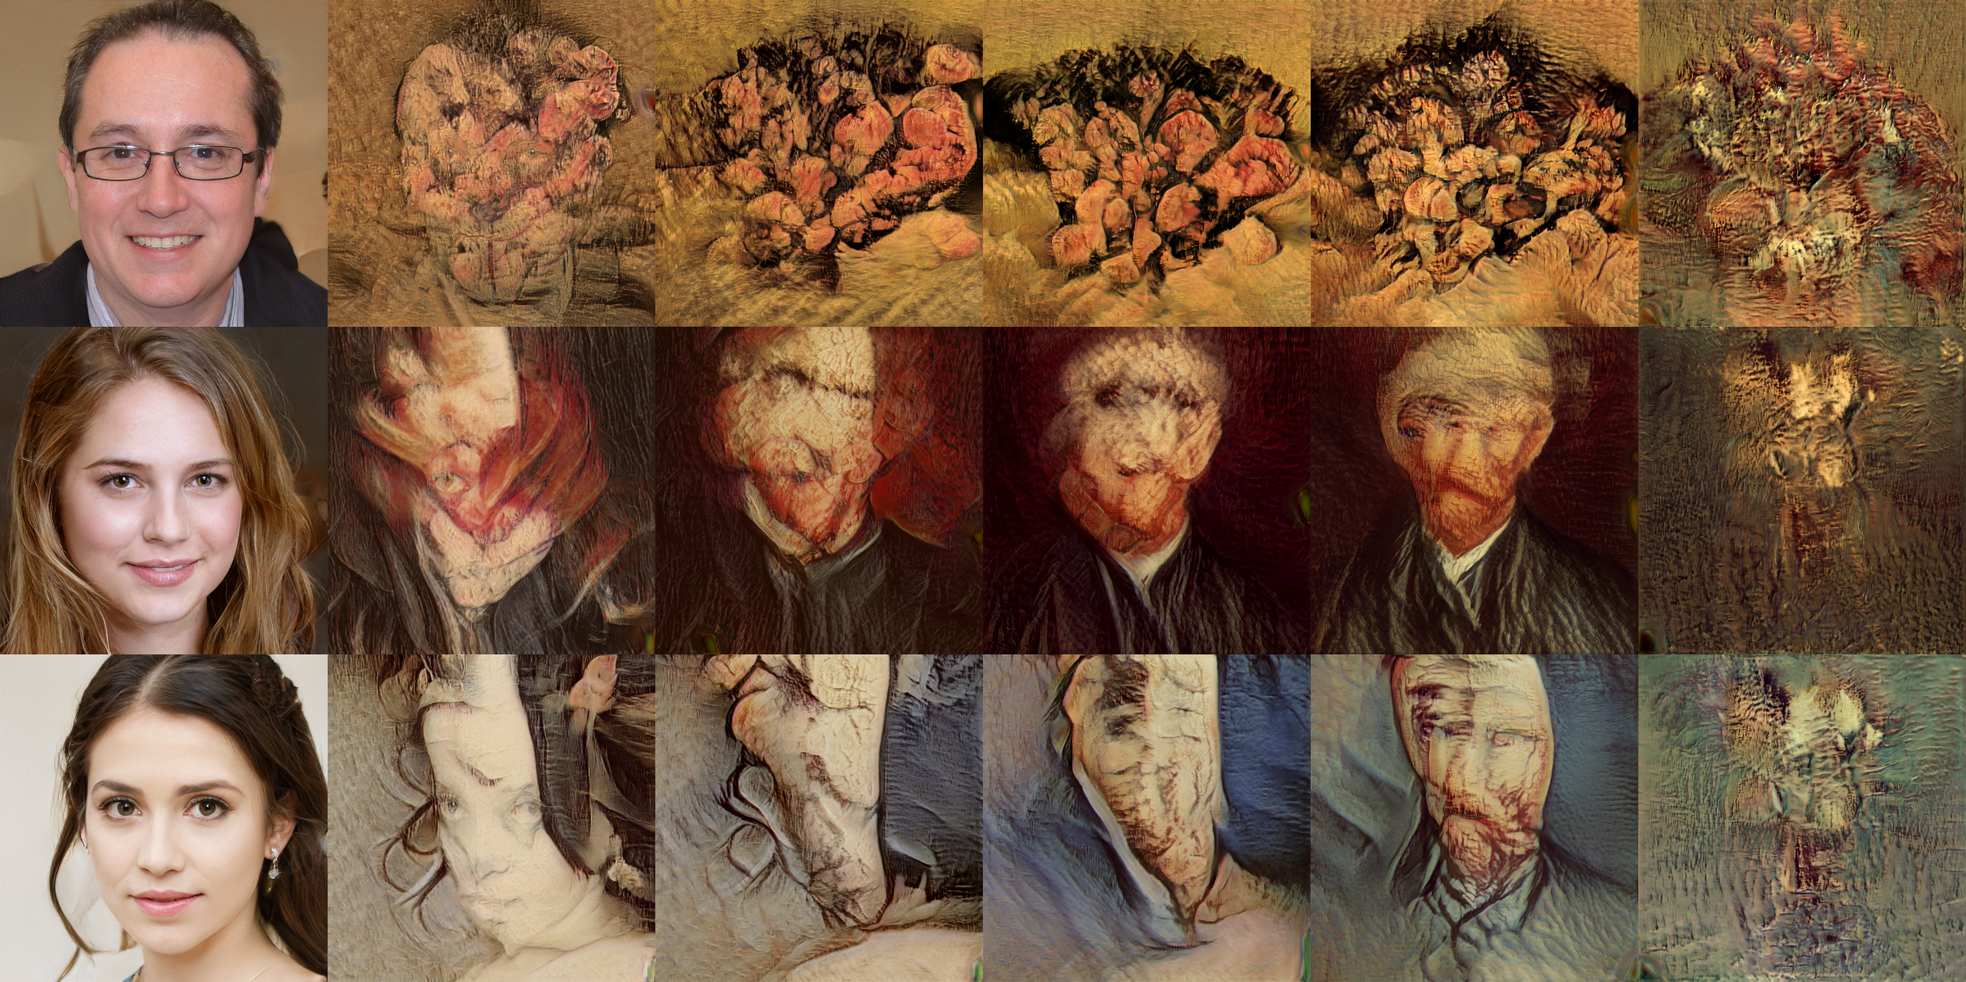
\includegraphics[width=\linewidth]{report/img/morphing.png}
    \caption{Generated images over the course of training the constant-sized StyleGAN instance. Every row corresponds to a randomly generated latent code, every column corresponds to a training tick.}
    \label{fig:sample_resumed}
\end{wrapfigure}

Figure \ref{fig:sample_restarted} shows sampled images from the progressively growing StyleGAN instance (also referred to as `training restarted' from here) over the course of training. Since this rendition of the network starts off with generating lower-resolution images, it is faster to train, hence it can do more ticks over the same training period; only a few ticks are showcased here for clarity. The first column again shows the faces generated by the original network, while in the second column the resolution is reset to 8x8 and increases from there. As training progresses, the pixelated blobs of color slowly coalesce into resemblances of flowers (first and second row) and landscapes (third row).

\begin{figure}
    \centering
    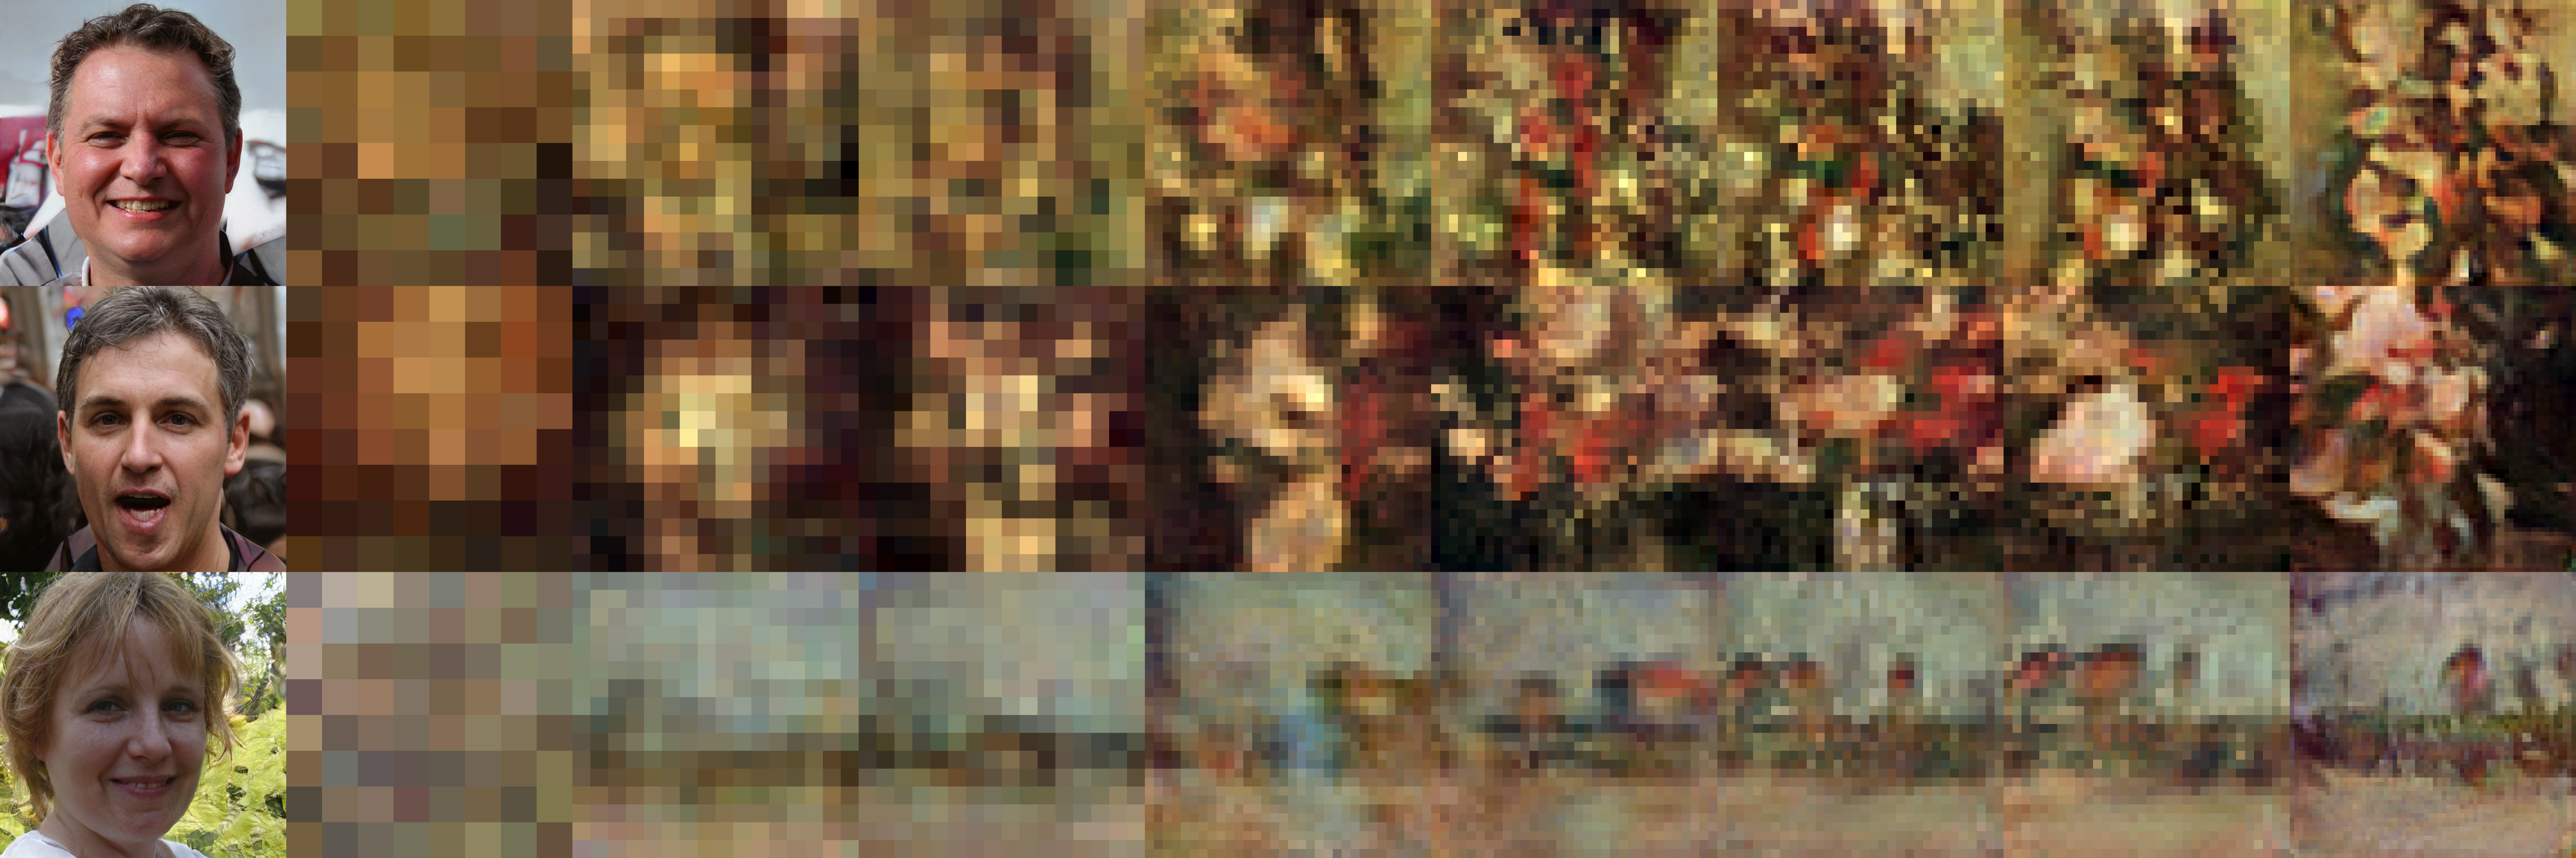
\includegraphics[width=0.8\linewidth]{report/img/retrain_morphing.png}
    \caption{Generated images over the course of training the growing StyleGAN instance. Every row corresponds to a randomly generated latent code, every column corresponds to a training tick.}
    \label{fig:sample_restarted}
\end{figure}

To also evaluate the progress of the StyleGAN instances quantitatively, the FID has been calculated for all training ticks of both instances (see Figure \ref{fig:fids}). The StyleGAN instance for which training was resumed shows a gently declining FID for the first three ticks, which then rises rapidly. Especially the high FID in the last tick matches well with the last column of Figure \ref{fig:sample_resumed} that has lost some of its resemblance to Van Gogh paintings.

As for the StyleGAN instance whose training schedule was reset, FIDs are higher overall than the instance for which the schedule was simply resumed, but the descend of the FID over training ticks is more persistent. There seem to be two moments at which the FID takes a relatively large step downwards. These descents seem to correspond to the ticks in which the resolution is increased, namely from 8x8 to 16x16 and from 16x16 to 32x32.

\begin{figure}
    \centering
    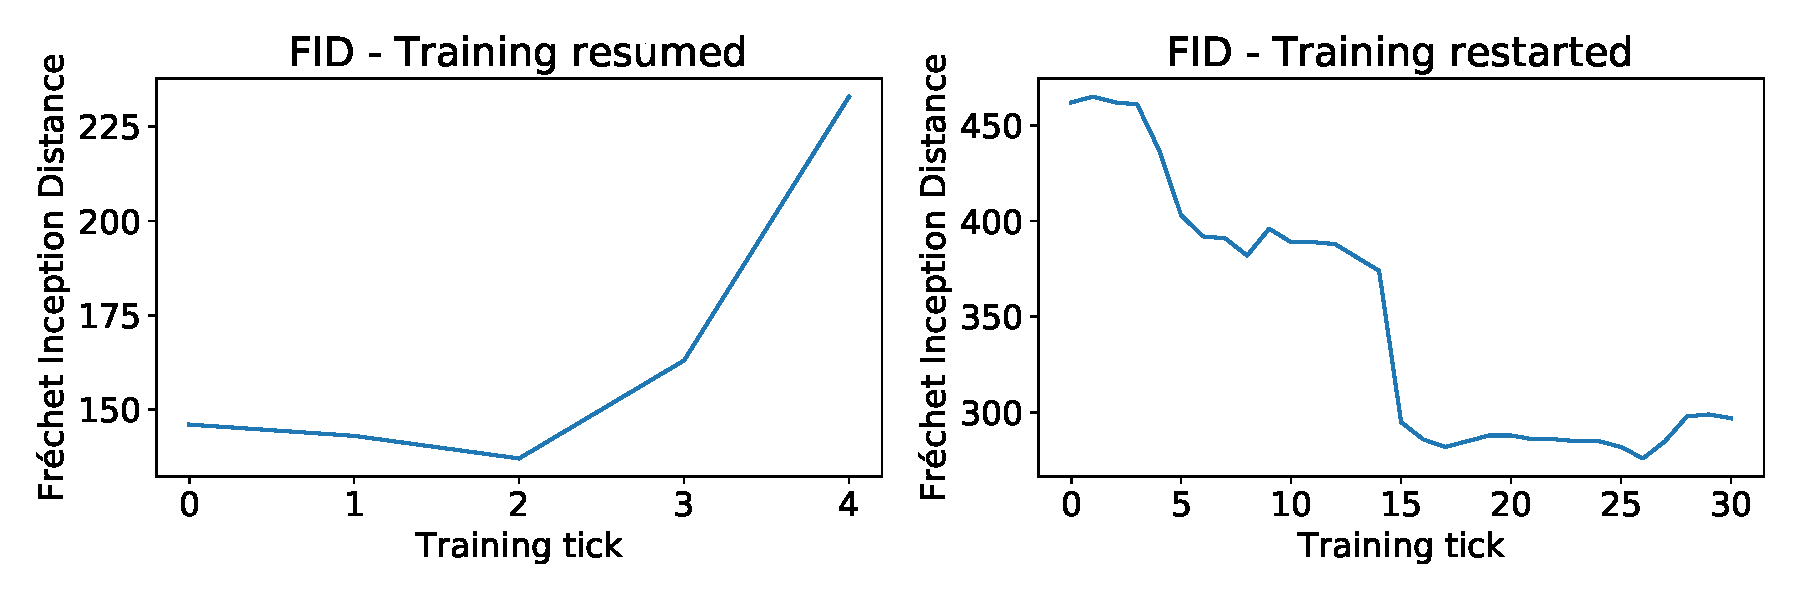
\includegraphics[width=\linewidth]{report/img/fids.pdf}
    \caption{FIDs of the constant-sized (left) and the progressively grown (right) StyleGAN instances. Ticks represent having trained on a number of images that depends on the training schedule; a tick is therefore not the same as what is commonly referred to as an epoch (an entire pass through the training data). The FID of the final state of the StyleGAN instance provided by \cite{karras2019stylebased}, that would precede the FID of tick 0, is \textit{not} included in the figures to allow for easier comparisons.}
    \label{fig:fids}
\end{figure}

\section{Conclusion}

We have trained two types of GANs, DCGAN and StyleGAN, on a dataset of paintings by Van Gogh with the aim of developing a network which is able to generate new paintings that have a style similar to Van Gogh's. Of the two, StyleGAN gave the most promising results. While the pretrained (constant-sized) instance in general gave better results than the progressively grown network in terms of the FID, we note that it appears to be prone to overfitting as the FID quickly grows after half a day of training. This is also visible in the results: the paintings produced in later epochs look worse than those created after half a day of training. The trend of the FID of the progressively grown StyleGAN on the other hand steadily decreases throughout the course of training. It would have been worthwhile to train this network for even longer to observe the minimal FID we could achieve, and compare this to the best fit produced by the constant-sized StyleGAN instance.

While the final results do not portray humans or landscapes accurately, we are pleased with the generated paintings, which definitely show similarity to Van Gogh's work in terms of colour usage, topics, and style.

% something about plug and play?


% NON-BNAIC STYLE
% \printbibliography
% \end{document}

% BNAIC STYLE
\newpage
\bibliographystyle{plain}
\bibliography{bibliography}
\end{document}


